% Author: Alexander Feng

\qns{RLC Bandstop Filter}

One way to compose a bandpass filter is by combining a low pass and high pass filter via a buffer.
Another way to compose a bandpass is to use a RLC circuit of the following form:

\begin{figure}[h!]
\begin{center}
\begin{circuitikz}[american]
    \node[ground](g){};
    \draw (g) to[sV, l = $V_{in}(t)$] ++ (0, 3) coordinate(input);
    \draw (input) -- ++(1, 0) to[C, l = $C$] ++ (0.5, 0) coordinate(capacitor);
    \draw (capacitor) -- ++(0.5, 0) to[L, l = $L$] ++(2, 0) coordinate(output) -- ++(1, 0) node[ocirc]{$ . V_{out}(t)$};
    \draw (output) to[R, l = $R$] ++(0, -3) node[ground]{};
\end{circuitikz}
\end{center}
\caption{RLC Bandpass Filter}
\end{figure}

Let's explore what happens when swap the location of the resistor with the location of the capacitor and inductor.

\begin{figure}[h!]
% Author: Alexander Feng Fall 2020
\begin{center}
\begin{circuitikz}[american voltages]
    \draw node[ground]{} (0,0) to[sV, l = $V_{in}(t)$, invert]
    (0,3) -- (0.25, 3) to[R = $R$] (3, 3) -- (4, 3) node[ocirc]{$ . V_{out}(t)$};
    \draw (3,3) to[C, C = $C$] (3, 1.5) to[L, L = $L$] (3,0) node[ground]{};
\end{circuitikz}
\end{center}

\caption{Unknown Behavior}
\end{figure}

\begin{enumerate}

\qitem
Write out the transfer function of figure 2.

\meta{
See if you can get students to guess what the behavior will ultimately be based on the topology of the circuit and what their knowledge of resonancy tells them so far.
In particular, during resonancy, the impedance of circuit elements cancel each other and cause a short.
In the bandpass, this results in $Vout(t)$ being directly connected to the voltage source.
In the bandstop, it results in a short to ground!
}

\sol{
Note that $j = -\frac{1}{j}$.
This can be proved by multiplying both sides by $j$.
Thus,
\begin{align*}
H_{notch}(j\omega) = \frac{j(L\omega - \frac{1}{C\omega})}{R + j(L\omega - \frac{1}{C\omega})}
\end{align*}
}

\qitem
What is the magnitude of the transfer function?

\sol{
\begin{align*}
\left | H_{notch}(j\omega) \right | =
\frac{\sqrt{(L\omega - \frac{1}{C\omega})^{2}}}{\sqrt{R^{2} + (L\omega - \frac{1}{Cw})^{2}}}
\end{align*}
}

\qitem
Sketch the magnitude of this transfer function.

\sol{
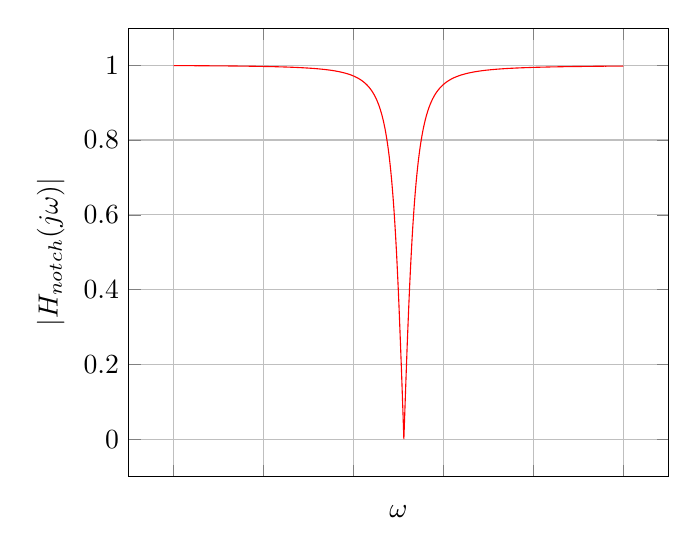
\begin{tikzpicture}
\begin{axis}[
xlabel={$\omega$},
ylabel={$|H_{notch}(j\omega)|$},
grid=major,
xticklabels = {}]
\addplot[domain=250:500, color = red, samples = 550]  {(((0.07 * x - ((1)/(0.0001 * x)))^2)^0.5)/((1 + ((0.07 * x) - (1)/(0.0001 * x))^2)^0.5)};
\end{axis}
\end{tikzpicture}

Notice that the magnitude of the transfer function is approximately one outisde of some very small region.
}

\qitem
When is the magnitude of the transfer function zero?
When is it one?

\sol{
The magnitude of the transfer function is zero precisely when
\begin{align*}
L\omega = \frac{1}{C\omega}
\end{align*}
}

\qitem
How would you describe the behavior of this circuit?
Why do you think circuits with this type of circuit behavior are classified as notch/bandstop filters?
Why is this specific filter called a \emph{resonsant} bandstop filter?


\sol{
The circuit's behavior can be thought of as the complement or opposite to the bandpass filter.
While the bandpass filter allows a range of frequencies through, the bandstop/notch stops a particular range of frequencies from passing through.
This is also why it'd be called bandstop or notch.
Bandstop is opposite of bandpass.
Notch comes from how the graph of the magnitude looks like there's a notch.
This filter is a specific type of bandstop filter in that it's resonant.
Resonance occurs when at a specific frequencies, the impedances of circuit elements cancel each other.
For this circuit, this occurs when $L\omega = \frac{1}{C\omega}$.
}




\end{enumerate}
